\documentclass[12pt,a4paper]{article}
\usepackage[utf8]{inputenc}
%referencing >>>>>>>>
\usepackage{amsmath}
\usepackage[english]{babel}
\usepackage[style=authoryear-ibid,backend=biber]{biblatex}
\addbibresource{bibliography.bib}% Syntax for version >= 1.2
%for minted>>>>>
\usepackage{minted}
\usemintedstyle{colorful}
%others >>>>>>>>
\usepackage{amsmath}
\usepackage{graphicx}
\usepackage{float}
\usepackage[center]{caption}
\usepackage[normalem]{ulem}
\usepackage{longtable}
\usepackage{comment}
\usepackage{array}
\usepackage{soul}
\usepackage{fancyhdr}
\usepackage{adjustbox}
\usepackage{amsmath}
\usepackage{amssymb}
\usepackage{zed-csp}
\usepackage{geometry}
%for links >>>>>>
\usepackage{hyperref}

\usepackage{csquotes}% Recommended
\usepackage{listings}

\usepackage{xcolor}



%New colors defined below
\definecolor{codegreen}{rgb}{0,0.6,0}
\definecolor{codegray}{rgb}{0.5,0.5,0.5}
\definecolor{codepurple}{rgb}{0.58,0,0.82}
\definecolor{backcolour}{rgb}{0.95,0.95,0.92}

%Code listing style named "mystyle"
\lstdefinestyle{mystyle}{
  backgroundcolor=\color{backcolour}, commentstyle=\color{codegreen},
  keywordstyle=\color{magenta},
  numberstyle=\tiny\color{codegray},
  stringstyle=\color{codepurple},
  basicstyle=\ttfamily\footnotesize,
  breakatwhitespace=false,         
  breaklines=true,                 
  captionpos=b,                    
  keepspaces=true,                 
  numbers=left,                    
  numbersep=5pt,                  
  showspaces=false,                
  showstringspaces=false,
  showtabs=false,                  
  tabsize=2
}

%"mystyle" code listing set
\lstset{style=mystyle}

\PassOptionsToPackage{hyphens}{url}\usepackage{hyperref}
\hypersetup{
    colorlinks=true,
    linkcolor=black,     
    urlcolor=blue,
    citecolor = black
}
\urlstyle{same}
	
\graphicspath{ {img/} }

\title{Report title}
\author{Zan Zver}
\date{Report Date }

%\documentclass[border=0.125cm]{standalone}
\usepackage{tikz}
\usetikzlibrary{positioning}
\newcommand{\latex}{\LaTeX\ }
\newcommand{\authorName}{Zan Zver}
\newcommand{\authorID}{18133498}
\newcommand{\reportTitle}{Deep learning dataset description and solution}
\newcommand{\degreeAward}{BSc (Hons) in Computer and Data Science } 
%\documentclass{article}
\usepackage{booktabs}% http://ctan.org/pkg/booktabs
\newcommand{\tabitem}{~~\llap{\textbullet}~~}

\begin{document}
\DeclareGraphicsExtensions{.jpg,.png,.gif,.pdf,.jpeg}
\begin{titlepage}
   \begin{center}
       CMP6228 – Deep Neural Networks
       \vspace*{0.5cm}

       \huge\textbf{\reportTitle} 

       \vspace{0.5cm}
        Coursework Assignment Report
            
       \vspace{1.5cm}

       \authorName \\
       \authorID\\
       \vspace{0.5cm}
       \large{Word count: 2012}


       \vfill
            
       \vspace{0.8cm}
     
       \begin{figure}[htp]
        \centering
        
\includegraphics{logo}
        \end{figure}
            
       \large{Faculty of Computing, Engineering and the Built Environment \\
       Birmingham City University \\}
            
   \end{center}
\end{titlepage}
\pagestyle{fancy}
\fancyhf{}
\rhead{
\includegraphics[width = 3.3cm]{header.jpg}}
\lhead{\footnotesize BIRMINGHAM CITY UNIVERSITY \\ SCHOOL OF COMPUTING AND DIGITAL TECHNOLOGY}
\rfoot{Page \thepage}
\newgeometry{top=110pt}
\setlength{\headsep}{50pt}

\tableofcontents

\listoftables

\listoffigures

\lstlistoflistings

\section{Introduction} %1
This report covers text prediction of chocolate ratings. The report describes dataset, its properties and a bit of cleaning as well. Since text prediction is not new, some related work is presented highlighting the inspiration for this project. In the last section more information about the model can be found including what data is going to be used and what the construction of the model is going to be. %1

\section{Problem statement}
The company \parencite{web:FlavorsOfCacao} has build modest dataset that describes chocolate rating. Their goal is for users to see the rating and decide to buy or not chocolate based on the rating.

So, what would the perfect chocolate be? It takes time, effort and finance to produce chocolate. To mitigate that, we can use neural networks to predict chocolate bar ratings and potentially discover the perfect conditions for chocolate bars. %2

\section{Proposed method}
To overcome the problem, we have chosen Python as programming language with Keras \parencite{web:AboutKeras} being main NN library in use. Since we need computation power, Google Colab \parencite{web:AboutGoogleColab} is being used as development platform. With that in mind, we can split the project into 11 main subsections.

\subsection{Import libraries}
As noted from before, main library used for our project is Keras. But, we need to do some data processing and for that we need other libraries (sklearn, numpy, pandas) and drawing the charts (matplolib).
\begin{lstlisting}[language=Python, caption=Import libraries]
import pandas as pd 
from sklearn.model_selection import KFold
import keras
import tensorflow as tf
from sklearn.preprocessing import OneHotEncoder
from keras.models import Sequential
from keras.layers import Dense
import numpy as np
from sklearn import preprocessing
from sklearn.preprocessing import StandardScaler
from sklearn.model_selection import train_test_split
import matplotlib.pyplot as plt
import seaborn as sns
from keras import layers
from keras import models
from keras import regularizers
from keras import optimizers
from sklearn.preprocessing import LabelEncoder 
from keras.utils import np_utils
from sklearn.metrics import multilabel_confusion_matrix
from sklearn.metrics import classification_report
from sklearn.metrics import confusion_matrix, ConfusionMatrixDisplay
import warnings
\end{lstlisting}

\subsection{Import the data}
Data is being directly imported from Kaggle to Google Colab. This is done with the help of their API \parencite{web:KaggleAPI}. So, first step is to create local (to Colab) dictionary (with the name of kaggle). Next, we move our API keys from Google Drive to our new folder. Now we change permissions of the keys so they can be read. After that, we download the dataset and we can see it saved locally. More information on the dataset can be found on appendix A1: About the data.
\begin{lstlisting}[language=Python, caption=Import the data]
! mkdir ~/.kaggle #create local kaggle folder
! cp /content/drive/MyDrive/Kaggle/kaggle.json ~/.kaggle/ #move auth key from one drive to temp folder
! chmod 600 ~/.kaggle/kaggle.json #use auth key
! kaggle datasets download rtatman/chocolate-bar-ratings -f flavors_of_cacao.csv #download the file from kaggle and unzip it while it is downloading
\end{lstlisting}

\subsection{Save data to pandas}
Now that we have the data saved locally (as CSV), we can access it. With Python, we save it to Pandas dataframe so we can modify it later.
\begin{lstlisting}[language=Python, caption=Save data to pandas]
cacao_dataframe_full=pd.read_csv('/content/flavors_of_cacao.csv')
\end{lstlisting}

\subsection{Filter the data}

There are some attributes in the dataset that are not useful for our case. Due to that, we are going to remove them.
\begin{lstlisting}[language=Python, caption=Remove attributes]
cacao_dataframe = cacao_dataframe_full
del cacao_dataframe["Company\xa0\n(Maker-if known)"]
del cacao_dataframe["REF"]
del cacao_dataframe["Review\nDate"]
\end{lstlisting}
Replace new lines (\textbackslash n) with spaces.
\begin{lstlisting}[language=Python, caption=Remove spaces]
cacao_dataframe.columns = cacao_dataframe.columns.str.replace
                                      ("\n", ' ', regex=True) 
\end{lstlisting}
Data in attribute "Cocoa Percent" has \% symbol next to the numeric value. This is something that needs to be changed, therefore all of the \% symbols are going to be removed from the attribute. 
\begin{lstlisting}[language=Python, caption=Remove symbols]
cacao_dataframe2 = pd.DataFrame(
             cacao_dataframe["Cocoa Percent"].str.replace("%",""))
cacao_dataframe.drop(["Cocoa Percent"], axis=1, inplace=True)
cacao_dataframe = cacao_dataframe.join(cacao_dataframe2)
\end{lstlisting}
While developing the code, we found out that our dataset is not big enough (in terms of records). This was clearly marked when we figured out that we only have 2 ratings that are marked as 5. To combat this, we have multiplied the whole dataset by 10. With that in mind, we still have the same ratio between results, it just makes it simpler to avoid facing wrong sizes upon fitting data to the model. Alternative would be to do data augmentation.
\begin{lstlisting}[language=Python, caption=Expend data]
cacao_dataframe_full = cacao_dataframe_full.loc
                        [cacao_dataframe_full.index.repeat(10)]
cacao_dataframe_full = cacao_dataframe_full.reset_index(drop=True)
\end{lstlisting}
While we did some data inspection, there seems to be data that is not unified. To combat this, all of the ratings are "rounded" the same way.
\begin{lstlisting}[language=Python, caption=Fix ratings]
def fix_ratings(rating):
    if rating < 0.5: 
        return 0.0 
    elif rating < 1.5: 
        return 1.0 
    elif rating < 2.5: 
        return 2.0
    elif rating < 3.5: 
        return 3.0
    elif rating < 4.5: 
        return 4.0 
    elif rating < 5.5: 
        return 5.0
    else:
        return 0.0
  
cacao_dataframe_full["Rating"] = 
    cacao_dataframe_full["Rating"].apply(lambda x: fix_ratings(x))
\end{lstlisting}

\subsection{One hot encoding of the data}
In our dataset, we have 6 attributes. 2 of them are of numeric type (Cocoa Percent and Rating), the other 4 are string types. With that in mind, we cannot do neural network operations on such dataset without some modifications.

To overcome the problem, we use one hot encoding for encoding the data\parencite{jie2019one}. What one hot encoding does, it binary encodes words into the dataframe. For example, if chocolate would have origin in UK, attribute would be created with the name of UK and all of chocolates with origin of UK would have 1 as a value and others would have 0.

In the code block bellow, we can see how we are encoding the data. First empty dataframe is build that will store the data and then the function is build that will encode the data. Next, we pass in our dataframe to be encoded and save it as encoded dataframe. In last step, we remove original attributes since they are not needed anymore.

\begin{lstlisting}[language=Python, caption=One hot encoding of the data]
encoded_dataframe = pd.DataFrame()
encoder = OneHotEncoder(handle_unknown='ignore')
def encodeRow(df, columnName):
    encoder_df = pd.DataFrame(encoder.fit_transform(df[columnName]).toarray())
    newNames= []
    for x in encoder.get_feature_names_out():
       x = x.replace("_", " ")
       x = x.rstrip()
       x = x.replace('\n', "_")
       x = x.replace(' ', "_")
       newNames.append(x)
    encoder_df.columns = list(newNames)
    return encoder_df

encoded_dataframe = cacao_dataframe_full.join(
                        encodeRow(cacao_dataframe_full,[
                            "Specific Bean Origin or Bar Name",
                            "Company Location", 
                            "Bean Type", 
                            "Broad Bean Origin"]
                        ))

encoded_dataframe.drop([
                "Specific Bean Origin or Bar Name",
                "Company Location",
                "Bean Type",
                "Broad Bean Origin"],
                axis=1, inplace=True)
\end{lstlisting}

\subsection{Split the data - X, y}
Now that we have the dataframe encoded we can split it up to X (features) and y (target). In the code block bellow, we can see X is collection of attributes from encoded dataframe that are indexed 1 and above. Opposite to that, y is single attribute from encoded dataframe that has index 0.
\begin{lstlisting}[language=Python, caption=Split the data - X and y]
X = encoded_dataframe.iloc[:,1:len(encoded_dataframe.columns)]
y = encoded_dataframe.iloc[:,0:1]
\end{lstlisting}

\subsection{Split the data - k-fold}
Next step is to split the data again but into 3 sections: train, test and validate. This can be done in a number of different ways, but one of the most efficient ways is k-fold cross validation \parencite{rodriguez2009sensitivity}.
What k-fold does, is it splits the data into k (number) of sections. With this, we can have the best ratio between train, test and validate.

The code block bellow is enabling us to do k-fold. First, we define parameters of k-fold into the variable of kf. Next, the function (kFoldValidation) is written that will split the data upon being called.
\begin{lstlisting}[language=Python, caption=Create k-fold function]
kf = KFold(n_splits = 10, shuffle = True, random_state = 6)
def kFoldValidation(df):
  result = next(kf.split(df), None)
  train = df.iloc[result[0]]
  test =  df.iloc[result[1]]
  return train, test
\end{lstlisting}
Now that we have our k-fold function sorted, we can use it. First, we split the data into two sections: 1) train and 2) validation and testing. Next step is to split second section apart into 2.1) validation and 2.2) testing. % maybe add that section 1 is the biggest
\begin{lstlisting}[language=Python, caption={Split the data to train, test and validate}]
X_train, X_val_and_test = kFoldValidation(X)
y_train, y_val_and_test = kFoldValidation(y)
X_val, X_test = kFoldValidation(X_val_and_test)
y_val, y_test = kFoldValidation(y_val_and_test)
\end{lstlisting}
The data is in the format of Pandas dataframe until now. This is something that needs to be changed in order for model to process the data. That is why, we have converted the data to numpy array. 
As seen in the code block bellow, data is also being transformed. Y (target) data is being encoded with label encoder since ratings (1-5) are potential labels. With X (input) data, this is being scaled based on the encoded data.
\begin{lstlisting}[language=Python, caption={Reshape the data to fit the model}]
sc = StandardScaler(with_mean=False)
sc.fit(X_train)

le = LabelEncoder()
le.fit(y_train)

X_train_transf = sc.transform(X_train)
X_test_transf = sc.transform(X_test)
X_val_transf = sc.transform(X_val)

y_train_cat = np_utils.to_categorical(le.transform(y_train))
y_test_cat = np_utils.to_categorical(le.transform(y_test))
y_val_cat = np_utils.to_categorical(le.transform(y_val))
\end{lstlisting}

\subsection{Build Neural Network}

\subsubsection{Model theory}
Plan for the model is to have 5 types of inputs (represented in \emph{Figure 1}). Although final (input) number is not going to be 5, rather it is going to be based on encoded cases (1242 in our case).
The output layer is expected to predict ratings. This should be a number in the range of 1 (the worse) to 5 (the best).
\newline
Inputs (X) for the model are:
\begin{itemize}
  \item I\textsubscript{1} $\Rightarrow$ Specific Bean Originor Bar Name,
  \item I\textsubscript{2} $\Rightarrow$ CocoaPercent,
  \item I\textsubscript{3} $\Rightarrow$ CompanyLocation,
  \item I\textsubscript{4} $\Rightarrow$ BeanType,
  \item I\textsubscript{5} $\Rightarrow$ Broad BeanOrigin.
\end{itemize}
Output (y) for the model is:
\begin{itemize}
  \item O\textsubscript{1} $\Rightarrow$ Rating 1
  \item O\textsubscript{2} $\Rightarrow$ Rating 2
  \item O\textsubscript{3} $\Rightarrow$ Rating 3
  \item O\textsubscript{4} $\Rightarrow$ Rating 4
  \item O\textsubscript{5} $\Rightarrow$ Rating 5
\end{itemize}
\subsubsection{Constructing the model}
In the model construction, different parameters were tested. At the end, the parameters (and hyper parameters) that yielded the best results are:
\begin{itemize}
    \item number of units: 200, 100 and 50
    \begin{itemize}
        \item In the first layer, we do start with 200 units. As we progress, number of units is decreased in each hidden layer. This results in H1 being 200, H2 100 and H3 has only 50 units. In the last (output) layer, we only have 5 units (since ratings are 1-5).
    \end{itemize}
    
    \item batch size: 128
    \begin{itemize}
        \item Batch size of 64 was the starter and it was tested up to 256. After the batch size of 158, difference was minimal therefore this was the chosen number.
    \end{itemize}
    
    \item number of epochs: 100
    \begin{itemize}
        \item For testing purposes, we have started with 20 epochs to save the time, but went with 100 for final product since the results are better with it.
    \end{itemize}
    
    \item learning rate: 0.00001
    \begin{itemize}
        \item Learning rates of 0.001, 0.0001, 0.00001 and 0.000001 were tested. At the end, 0.00001 gave the best results.
    \end{itemize}
    
    \item momentum
    \begin{itemize}
        \item This function is left disabled. After testing it, momentum of 0.2 and 0.3 brings the best results but if it is disabled (set to 0.0), results are even better.
    \end{itemize}
    
    \item dropout: 0.3 and 0.2
    \begin{itemize}
        \item First layer is using dropout of 0.3. After that, we have decreased dropout to 0.2 for the rest of hidden layers (H2 and H3).
    \end{itemize}
    
    \item activation function: LeakyReLU and softplus in last
    \begin{itemize}
        \item Input function and  hidden layers 1-3 (H1, H2 and H3) are using linear activation function. In the last layer, softplus converts vector to a distribution that can be used for predicting Ratings.
    \end{itemize}
    
    \item number of layers: 5
    \begin{itemize}
        \item Input layer
        \item Hidden layer 1
        \item Hidden layer 2
        \item Hidden layer 3
        \item Output layer
    \end{itemize}
    
    \item optimizer: RMSprop
    \begin{itemize}
        \item Diferent optimises were tested along the way. At the end, there were two candidates: RMSprop and SGD. After some testing RMSprop delivered slightly better results therefore it was chosen.
    \end{itemize}
    
    \item loss function: categorical crossentropy
    \begin{itemize}
        \item Loss function of choice is categorical crossentropy. This is due to our problem being predicting Ratings, therefore we have chosen that.
    \end{itemize}
    
    \item metrics: accuracy
    \begin{itemize}
        \item accuracy is not the only metrics used in industry, but it is the most well known. This is the reason for implementing it. Besides that, confusion matrix is being used as well (that is showcased at the end).
    \end{itemize}
    
\end{itemize}
\input{report/proposedMethod/buildNeuralNetwork/model}
\input{report/proposedMethod/buildNeuralNetwork/code}

\subsection{Test Neural Network}
To test the NN, we put the last batch of never seen data to it. This is test data. With that in mind, we can see our evaluation and determine if this is matching to the results from model training.
\begin{lstlisting}[language=Python, caption=Evaluate the model]
scores = model.evaluate(X_test_transf, y_test_cat, batch_size=128)
print("%s: %.2f%%" % (model.metrics_names[1], scores[1]*100))
\end{lstlisting}

\subsection{Calculate and display model results}
To calculate and display results, we first need to grab the data. We do this by getting history data that we have created from above.
\begin{lstlisting}[language=Python, caption=Create dictionary of history values]
history_dict = history.history
history_dict.keys()
\end{lstlisting}
This step is not necessary, but it is convenient. What we do is, extract values based on keys and save it to local variables.
\begin{lstlisting}[language=Python, caption=Save data from dict to local variables]
training_acc = history_dict['accuracy']
val_acc = history_dict['val_accuracy']

training_loss = history_dict["loss"]
val_loss = history_dict["val_loss"]
\end{lstlisting}
In the next step, we plot our first graph as training and validation accuracy.
\begin{lstlisting}[language=Python, caption=Plot training and validation accuracy]
epochs = range(1, len(val_acc) + 1)

plt.plot(epochs, training_acc, 'bo', label="Training Accuracy")
plt.plot(epochs, val_acc, 'b', label='Validation Accuracy')

plt.title('Plot training and validation accuracy')

plt.legend()
plt.show()
\end{lstlisting}
Finaly, we plot the last graph as training and validation loss.
\begin{lstlisting}[language=Python, caption=Plot training and validation loss]
epochs = range(1, len(training_loss) + 1)

plt.plot(epochs, training_loss, 'bo', label='Training Loss')
plt.plot(epochs, val_loss, 'b', label='Validation Loss')

plt.title('Plot training and validation loss')

plt.legend()
plt.show()
\end{lstlisting}

\subsection{Confusion matrix}
To evaluate the data (further), we are using confusion matrix \parencite{visa2011confusion}. This standard is popular in the industry. 
In the first code block, we are calculating multi label confusion matrix and displaying the results.
\begin{lstlisting}[language=Python, caption=Calculate confusion matrix]
warnings.filterwarnings('ignore')
preds = model.predict(X_test_transf)
preds = np.where(preds < 0.5, 0, 1)

target_names = ['Rating 1', 'Rating 2', 'Rating 3', 'Rating 4', 'Rating 5']
cm = multilabel_confusion_matrix(y_test_cat, preds)
print(classification_report(y_test_cat, preds, target_names=target_names))
\end{lstlisting}
Second code block is for visualise confusion matrix. Since we have multi label confusion matrix, each label (class) is visualised separately.
\begin{lstlisting}[language=Python, caption=Visualise confusion matrix]
f, axes = plt.subplots(1, 5, figsize=(20, 10))
axes = axes.ravel()
for i in range(5):
    disp = ConfusionMatrixDisplay(confusion_matrix(y_test_cat[:, i],
                                                   preds[:, i]),
                                  display_labels=[0, i+1])
    disp.plot(ax=axes[i], values_format='.4g')
    disp.ax_.set_title(f'Rating {i+1}')
    if i<10:
        disp.ax_.set_xlabel('')
    if i%5!=0:
        disp.ax_.set_ylabel('')
    disp.im_.colorbar.remove()

plt.subplots_adjust(wspace=0.10, hspace=0.1)
f.colorbar(disp.im_, ax=axes)
plt.show()
\end{lstlisting} %3

\section{Experimental Results}

% trainingAndValidationAccuracy.jpeg
% trainingAndValidationLoss.jpeg
% clculationConfusionMatrix.jpeg
% visualiseConfusionMatrix.jpeg
Model evaluation shows us accuracy of 93\% with test data.
\begin{figure}[H]
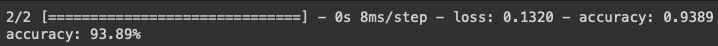
\includegraphics[scale=0.55]{img/evaluateModel.png}
\centering
\caption{Evaluation model results}
\end{figure}
Graph that represent accuracy over the time of epochs. As seen at the begging graph stars in 85\% and then raises to 90\% to 92\%. There is a bit of overfitting in the represented graph. Different methods were tried to reduce that but difference of 1\% to 2\% between training and validation is the best result that came out.
\begin{figure}[H]
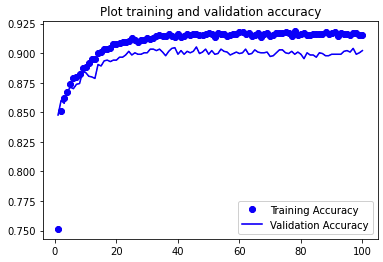
\includegraphics[scale=0.7]{img/trainingAndValidationAccuracy.jpeg}
\centering
\caption{Representation of training and validation accuracy}
\end{figure}
Representation of loss graph is showcasing training and validation difference. As the graph is showcasing, training and validation are on point.
\begin{figure}[H]
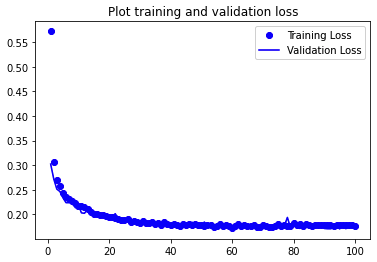
\includegraphics[scale=0.7]{img/trainingAndValidationLoss.jpeg}
\centering
\caption{Representation of training and validation loss}
\end{figure}
With the help of SkLearn library, multi label confusion matrix is calculated and shown. There are 4 things that are represented:
\begin{itemize}
    \item precision
    \item recall
    \item f1-score
    \item support
\end{itemize}
Calculations are done of micro, macro, weighted and samples. With that, we can see different calculations based on different scenarios.
\begin{figure}[H]
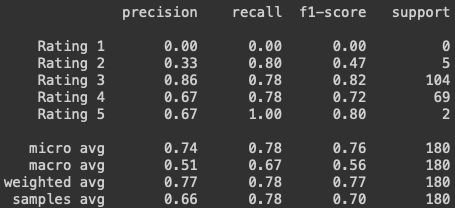
\includegraphics[scale=0.7]{img/clculationConfusionMatrix.jpeg}
\centering
\caption{Representation of calculation confusion matrix}
\end{figure}
Last figure represents multi label confusion matrix. Each label is represented separately. 
\begin{figure}[H]
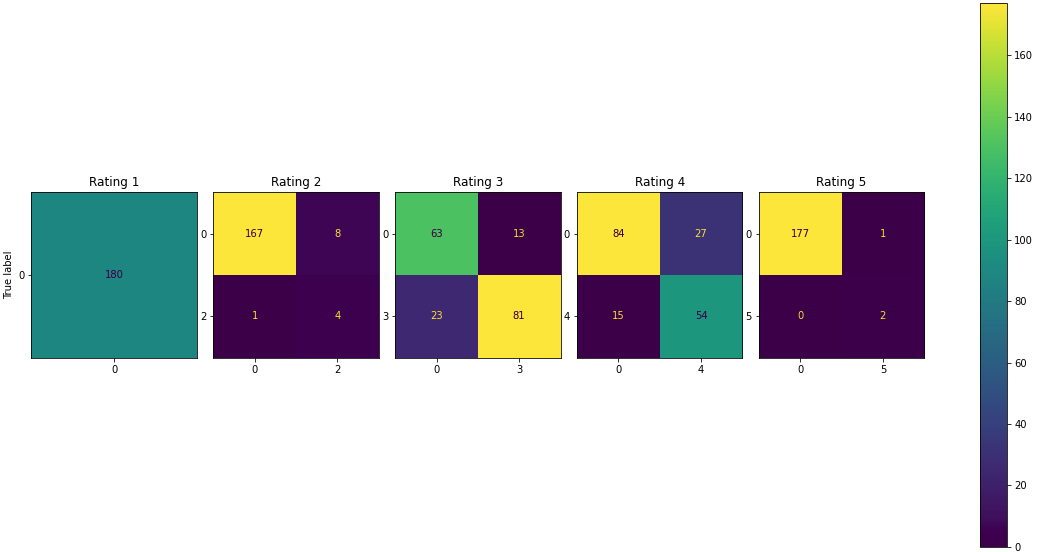
\includegraphics[scale=0.39]{img/visualiseConfusionMatrix.jpeg}
\centering
\caption{Representation of visualise confusion matrix}
\end{figure} %4

\section{Summary}
At the end of the report, we have successfully created a model that can predict chocolate ratings. With that, concept companies could base their new operations based on the predictions. 
The model is doing predictions in the code at the moment, this would not be user friendly in the industry. Due to this, we would need to implement some sort of GUI for better access.
Hypothetically, if the model would be used and efficient in the industry, if would need to be maintained. With that in mind, data drift can occur. For example, if a country X turns out to have the best conditions and a lot of chocolate industry moves to this, we would have our dataset filled with this country being the best. This can overflow the new locations therefore predictions can be offset.

Overall, there is still room for improvement but that is on the data side as well. For example, if we could get air pollution data, weather data, etc... quality of results would be better. In this report, data was representing kind of a bottleneck since results could be better if we had a bit more diverse dataset. From the model set, at the moment the simple sequential model is being used. If we would build some custom hidden layers, that could result in better accuracy since it would be tailored for our use case.
 %5

\section{Appendixes}
\subsection{A1: About the data}
Dataset is created by the company FlavorsOfCacao and can be found on Kaggle \parencite{web:FlavorsOfCacaoDataset}. The company goal is to provide independent chocolate ratings which could be displayed on chocolate bar. Idea they have is for the customer to compare two chocolates not on the price but on the rating. For example, customer would pick up chocolate A and chocolate B in the store, based on the rating customer can decide if chocolate is worth his money.
Dataset itself is build on 9 attributes and 1795 records (described in the table bellow).

\begin{table}[H]
  \centering
    \begin{tabular}{ |m{12em}|m{20em}| } 
     \hline
     Dataset attributes & Dataset description \\ 
     \hline
        Company (Maker-if known) &
        \tabitem Name of the company that is producing the chocolate (e.g.: Cadbury)  \\ &
        \tabitem Data type: string \\
     \hline
    Specific Bean Originor Bar Name &
        \tabitem Where chocolate bar was created \\ &
        \tabitem Data type: string \\
     \hline
    REF &
        \tabitem Value when review was entered in the database \\ &
        \tabitem Could be useful if we would be comparing chocolate over time, and how companies have evolved, other than that this attribute will be skipped \\ &
        \tabitem Data type: int \\
     \hline
    ReviewDate &
        \tabitem When the review has been released/added to the website \\ &
        \tabitem Data type: int \\
     \hline
        CocoaPercent &
        \tabitem What is the percentage of cocoa (darkness) in the chocolate \\ &
        \tabitem Data type: string \\
     \hline
        CompanyLocation &
        \tabitem Where is the company based from \\ &
        \tabitem Data type: string \\
     \hline
        Rating &
        \tabitem The mark from 1 (lowest) to 5 (highest) representing quality of the chocolate \\ &
        \tabitem Data type: float \\
     \hline
        BeanType &
        \tabitem Some chocolates do use bean combination, and this can be found here \\ &
        \tabitem Data type: string \\
     \hline
        Broad BeanOrigin &
        \tabitem Where is the broad geo-region of bean origin \\ &
        \tabitem Data type: string \\
     \hline
     
    \end{tabular}
\caption{Dataset attributes described}
\end{table} %6

\newpage

\section{References}
\printbibliography
\newpage

\end{document}